\documentclass{beamer}
\usepackage{amssymb}
\usepackage{amsthm}
\usetheme{CambridgeUS}
\providecommand{\mbf}{\mathbf}
\providecommand{\pr}[1]{\ensuremath{\Pr\left(#1\right)}}
\providecommand{\qfunc}[1]{\ensuremath{Q\left(#1\right)}}
\providecommand{\sbrak}[1]{\ensuremath{{}\left[#1\right]}}
\providecommand{\lsbrak}[1]{\ensuremath{{}\left[#1\right.}}
\providecommand{\rsbrak}[1]{\ensuremath{{}\left.#1\right]}}
\providecommand{\brak}[1]{\ensuremath{\left(#1\right)}}
\providecommand{\lbrak}[1]{\ensuremath{\left(#1\right.}}
\providecommand{\rbrak}[1]{\ensuremath{\left.#1\right)}}
\providecommand{\cbrak}[1]{\ensuremath{\left\{#1\right\}}}
\providecommand{\lcbrak}[1]{\ensuremath{\left\{#1\right.}}
\providecommand{\rcbrak}[1]{\ensuremath{\left.#1\right\}}}
\usepackage{amssymb,amsmath}

\renewcommand\thesection{\arabic{section}}
\renewcommand\thesubsection{\thesection.\arabic{subsection}}
\renewcommand\thesubsubsection{\thesubsection.\arabic{subsubsection}}
\numberwithin{equation}{subsection}
% Title page details: 
\title{AI1110 - ASSIGNMENT 4} 
\author{J. TUSHITA SHARVA - CS21BTECH11022}
\date{\today}
\logo{\large \LaTeX{}}


\begin{document}

% Title page frame
\begin{frame}
    \titlepage 
\end{frame}

% Remove logo from the next slides
\logo{}

% Outline frame
\begin{frame}{Outline}
    \tableofcontents
\end{frame}




\section{Question}
\begin{frame}{Question}
    \begin{block}{N.C.E.R.T Mathematics for class 12,Probability Chapter, Exercise 1, question 8}
        An instructor has a question bank consisting of
300 easy True/ False questions, 200 difficult True/
False questions, 500 easy multiple choice questions
and 400 difficult multiple choice questions. If a
question is selected at random from the question
bank, what is the probability that it will be an easy
question, given that it is a multiple choice question?
    \end{block}
\end{frame}

\section{Solution}
\begin{frame}{Given Information}
In the question, it was given that there were 
\begin{enumerate}
    \item 300 easy True/ False questions
    \item 200 difficult True/False questions
    \item 500 easy multiple choice questions
    \item 400 difficult multiple choice questions
\end{enumerate}
Additionally, it was also known that the random question picked was multiple choice question.\\
We have to find the probability  that it will be an easy question, given that it is a multiple choice question.
\end{frame}

\begin{frame}{Concepts}

\begin{block}{Formulas}
    \begin{align}
        \pr{E} = \frac{n(E)}{n(S)}\\
        \pr{E|F} = \frac{\pr{E,F}}{\pr{F}}
    \end{align}
\end{block}
    
\begin{alertblock}{Note:}
    We use the concept of Random Variables here. A random variable is a real valued function defined on the sample space. Since they are assigned to the outcome of the sample space, probabilities can be assigned to them.
\end{alertblock}

\end{frame}

\begin{frame}{Assigning Random Variables}

    \begin{alertblock}{Note:}
        This question has two simultaneous aspects to be covered:
        \begin{enumerate}
            \item Difficulty of the question \brak{Easy,\ tough}
            \item Type of Question \brak{T/F,\ MCQ}
        \end{enumerate}
        Therefore we shall use two different random variables X and Y.
    \end{alertblock}
    
    \begin{block}{Random Variable X : Assigned to the difficulty of the question}
        $X \in \cbrak{0, 1}$. \\ If $X = 0,$ the question is easy. Else difficult.\\
    \end{block}
    
    \begin{block}{Random Variable Y: Assigned to the type of question asked}
        $Y \in \cbrak{0, 1}$. \\ If $Y = 0,$ the question is a multiple choice question. Else, it is a True/ False question.
    \end{block}
    
\end{frame}

\begin{frame}{Probabilities using Random Variables}

    \begin{align}
    \pr{X = k} = 
      \begin{cases}
      \frac{8}{14}, & k = 0 \\
      \frac{6}{14}, & k = 1 
      \end{cases}
    \end{align}

\begin{figure}[!ht]
       \centering
       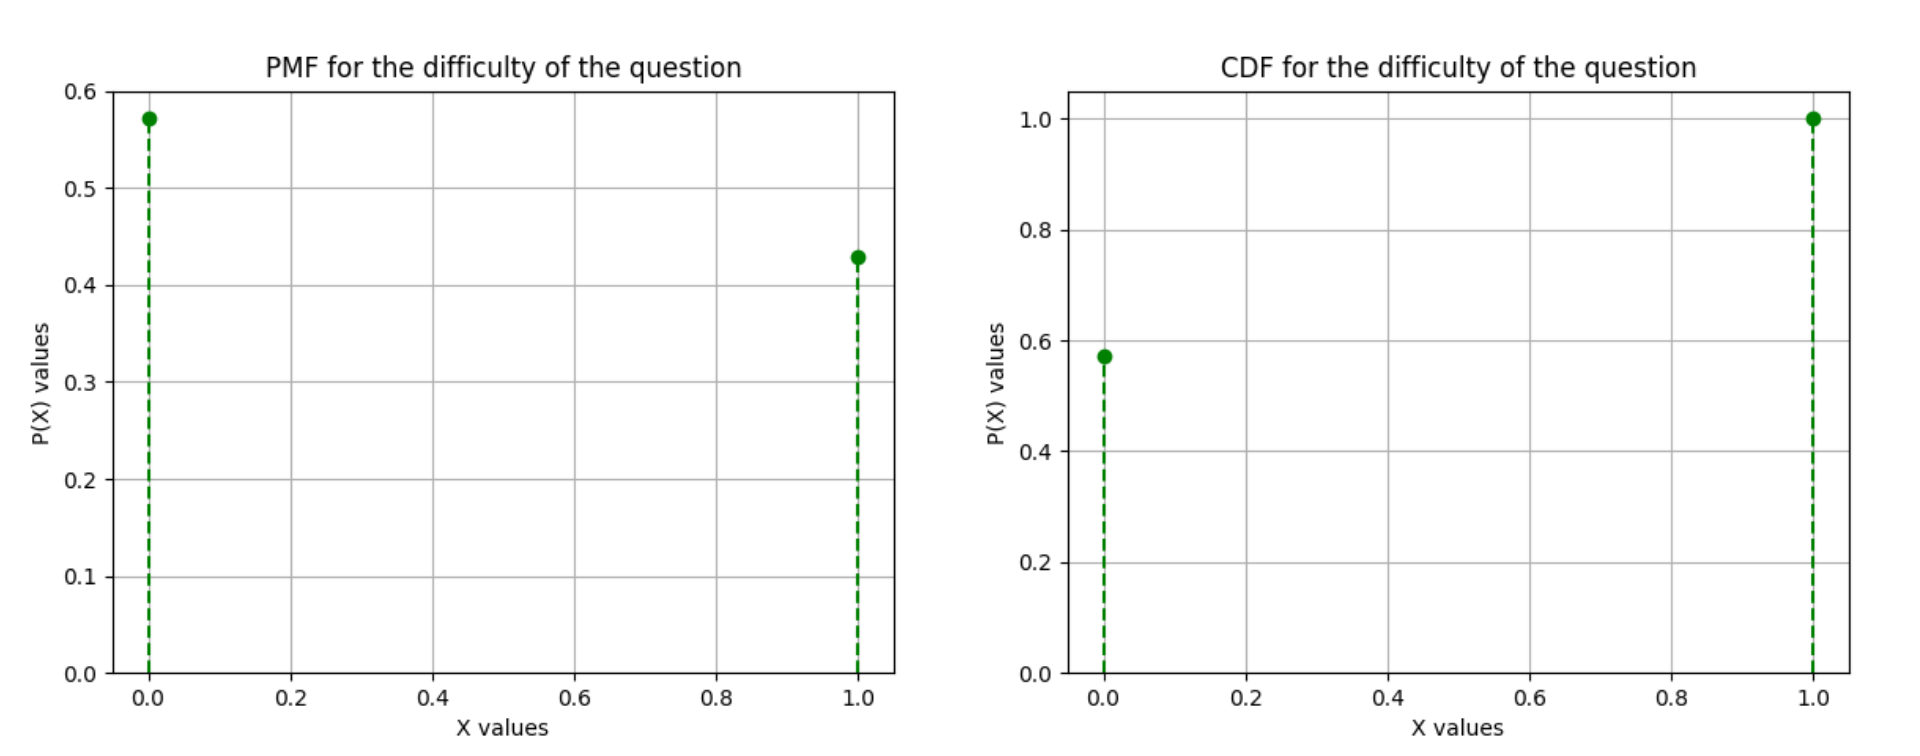
\includegraphics[width = 300pt]{CombinedDifficulty.png}
       \caption{PMF and CDF}
       \label{fig:Question Difficulty}
\end{figure}

\end{frame}

\begin{frame}{Probabilities using Random Variables}

\begin{align}
    \pr{Y = k} = 
      \begin{cases}
      \frac{5}{14}, & k = 0 \\
      \frac{9}{14}, & k = 1 
      \end{cases}
\end{align}

\begin{figure}[!ht]
       \centering
       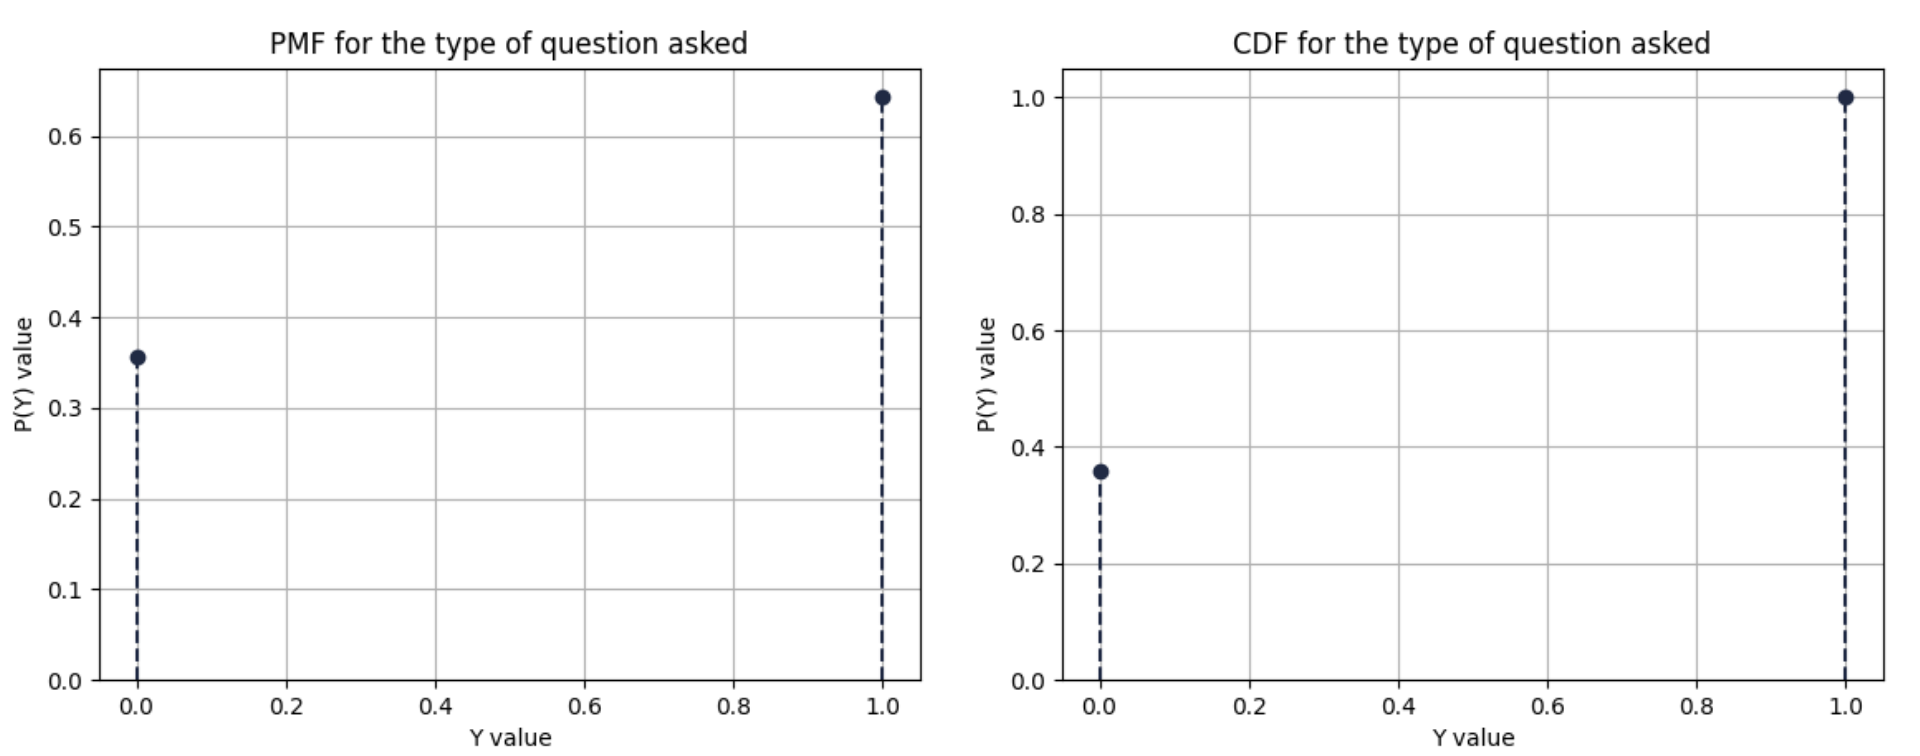
\includegraphics[width = 300pt]{CombinedPythonQuestionType.png}
       \caption{PMF and CDF}
       \label{fig:Question Difficulty}
\end{figure}
\end{frame}

\begin{frame}{Solution}
   We require the probability that it is an easy question given that it is a Multiple Choice Question.\\
i.e., We require $\pr{X = 0\ |\ Y = 1}$. We know that
\begin{align}
    \pr{X = 0} = \frac{8}{14}\\
    \pr{Y = 1} = \frac{9}{14}\\
   \pr{X = 0, Y = 1} = \frac{5}{14}
\end{align}

\pagebreak

Using the general formula for conditional probability, we have 

\begin{align}
    &\pr{X = 0\ |\ Y = 1} = \frac{\pr{X = 0, Y = 1}}{\pr{Y = 0}}&
\end{align}
\end{frame}

\begin{frame}{Solution}
    Substituting the values, we have:
\begin{align}
    \implies \pr{X = 0\ |\ Y = 1} = \frac{5/14}{9/14}\\
    \implies \pr{X = 0\ |\ Y = 1} = \frac{5}{9}
\end{align}

\begin{block}{Answer}
    Therefore, the probability that the question will be an easy one, given that it is a multiple choice question is $\displaystyle\frac{5}{9}$.
\end{block}

\end{frame}

\end{document}

